\begin{figure}[h]
      \centering   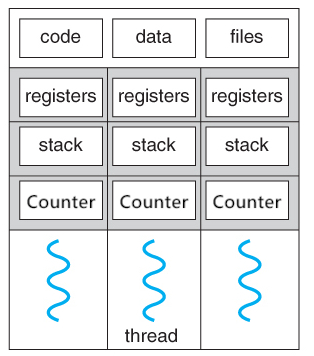
\includegraphics[scale=2]{./images/threads_01.jpeg}
\end{figure}

\begin{enumerate}
    \item zzz
    \item zzz
\end{enumerate}

\begin{myTableStyle}
    \begin{tabular}{ |m{8cm}|m{8cm}| } \hline
        User thread             &     Kernel Thread         \\ \hline
        Implemented by user     &     Implemented by OS.    \\ \hline
    \end{tabular}
\end{myTableStyle}
\vspace{0.08in}

\fillin[]



                TLB access time                     &   \(t_b\)         \\ \hline
                main memory access time             &   \(t_m\)         \\ \hline
                TLB access time                     &   \(t_b\)         \\ \hline
                TLB access time                     &   \(t_b\)         \\ \hline

\begin{lstlisting}

\end{lstlisting}

\lstinputlisting[language=Octave]{BitXorMatrix.m}

\begin{myTree}
  \node [circle,draw] [red] (node_a){root}
    child
    {
        node [circle,draw] (node_b) {b}
        child
        {
            node [circle,draw] (node_e) {e}
        }
        child
        {
            node [circle,draw] (node_f) {f}
        }
    }
    child
    {
        node [circle,draw] (node_d){d}
        child
        {
            node [circle,draw] (node_g) {g}
        }
        child
        {
            node [circle,draw] (node_h) {h}
        }
    };
\end{myTree}


\Theta  \omega  \Omega  \log_{a}b


oneparchoices

\begin{comment}

\begin{questyle}
  \question  zzz  (GATE-zzz)

  \begin{choices}
    \choice         zzz
    \choice         zzz
    \choice         zzz
    \choice         zzz
    \CorrectChoice
  \end{choices}
\end{questyle}

\begin{questyle}
  \question  zzz  (GATE-zzz)

  \begin{choices}
    \choice         zzz
    \choice         zzz
    \choice         zzz
    \choice         zzz
    \CorrectChoice
  \end{choices}
\end{questyle}

\begin{questyle}
  \question  zzz  (GATE-zzz)

  \begin{choices}
    \choice         zzz
    \choice         zzz
    \choice         zzz
    \choice         zzz
    \CorrectChoice
  \end{choices}
\end{questyle}

\begin{questyle}
  \question  zzz  (GATE-zzz)

  \begin{choices}
    \choice         zzz
    \choice         zzz
    \choice         zzz
    \choice         zzz
    \CorrectChoice
  \end{choices}
\end{questyle}

\begin{questyle}
  \question  zzz  (GATE-zzz)

  \begin{choices}
    \choice         zzz
    \choice         zzz
    \choice         zzz
    \choice         zzz
    \CorrectChoice
  \end{choices}
\end{questyle}

\begin{questyle}
  \question  zzz  (GATE-zzz)

  \begin{choices}
    \choice         zzz
    \choice         zzz
    \choice         zzz
    \choice         zzz
    \CorrectChoice
  \end{choices}
\end{questyle}

\begin{questyle}
  \question  zzz  (GATE-zzz)

  \begin{choices}
    \choice         zzz
    \choice         zzz
    \choice         zzz
    \choice         zzz
    \CorrectChoice
  \end{choices}
\end{questyle}

\begin{questyle}
  \question  zzz  (GATE-zzz)

  \begin{choices}
    \choice         zzz
    \choice         zzz
    \choice         zzz
    \choice         zzz
    \CorrectChoice
  \end{choices}
\end{questyle}

\begin{questyle}
  \question  zzz  (GATE-zzz)

  \begin{choices}
    \choice         zzz
    \choice         zzz
    \choice         zzz
    \choice         zzz
    \CorrectChoice
  \end{choices}
\end{questyle}

\begin{questyle}
  \question  zzz  (GATE-zzz)

  \begin{choices}
    \choice         zzz
    \choice         zzz
    \choice         zzz
    \choice         zzz
    \CorrectChoice
  \end{choices}
\end{questyle}

\begin{questyle}
  \question  zzz  (GATE-zzz)

  \begin{choices}
    \choice         zzz
    \choice         zzz
    \choice         zzz
    \choice         zzz
    \CorrectChoice
  \end{choices}
\end{questyle}

\begin{questyle}
  \question  zzz  (GATE-zzz)

  \begin{choices}
    \choice         zzz
    \choice         zzz
    \choice         zzz
    \choice         zzz
    \CorrectChoice
  \end{choices}
\end{questyle}

\end{comment}

